\section{Introduction}

\subsection{Chapter outline}

In this chapter, I explore the relationship between disease prevalence and infection intensity for helminth parasites. I challenge the standard negative binomial assumptions and briefly investigate the practical implications of such assumptions, particularly in conjunction with a range of mass drug administration (MDA) modelling assumptions. 

\section{Background}

As discussed in Chapter \ref{chap:STH}, disease prevalence ($P$) for helminth infections is often assumed to link to intensity (or mean worm burden, $M$) through a negative binomial distribution \cite{Anderson1992}. This is based on the knowledge that there is heterogeneity in the parasite burden between hosts, otherwise known as the aggregation of parasites within the host population. The derivation of this relationship is based on the assumption of a gamma-distributed infection risk combined with a Poisson distributed acquisition rate, giving the following analytical expression:

\begin{equation}
P = 1 - (1+M/k)^{-k}
\label{eqn:negbin1}
\end{equation}

Aggregation $k$ is expected to vary between settings, but is sometimes also taken as a function of $M$, linear or otherwise \cite{Norman2000_epifil, Anderson1992}. However, for modelling purposes aggregation is often considered constant for a particular region or setting.

This derivation has proved a highly powerful and useful tool in modelling helminth infections, however it is also considered by some as a non-ideal approximation, due to the increase in either biological or mathematical complexities often required to incorporate the negative binomial structure into models \cite{Yakob2014}. Converting results to prevalence also means that information is lost about the distribution of worm burden in the population, which is interlinked with the morbidity of disease and other important epidemiological factors. In particular, lower prevalence is associated with higher degrees of aggregation \cite{Truscott2019}.

However, unless the model is individual-based, prevalence measures are often used in the implementation of model simulations. For example, in vector-borne helminth infection models the force of infection from the host population to the vector population is often taken to be a function of the host prevalence rather than the mean worm burden, as it is necessary to include the probability of a vector biting an infectious individual. Ideally we would use a formulation based on $M$ rather than the host prevalence.

\section[LF]{Lymphatic filariasis force of infection}

If we consider the lymphatic filariasis (LF) model in Chapter \ref{chap:VEC}, then it is possible to describe such a formulation for the force of infection on the vector population as a function of $M$. To estimate host prevalence we consider the mf count per 20$\mu$l of blood in an individual as being distributed following a negative binomial distribution. From Anderson and May \cite{Anderson1992}, we have that the probability of $z$ parasites per 20$\mu$l of blood when sampling a random individual from the population is:
\begin{equation}
\mathbb{P}[z|M,k] = \binom{z+k-1}{z} \Big(1+\frac{M}{k}\Big)^{-k-z}\Big(\frac{M}{k}\Big)^z\,.
\label{eqn:negbin}
\end{equation}
Here $M$ is the mean mf count and $k$ is a descriptor of over-dispersion.

Take $A$ to be the ratio of mosquito feeding volume to 20$\mu$l, $A=($Feeding volume$)/20\mu$l, and $\eta$ to be the probability one ingested mf results in an L3 infection. Then, assuming a single hit model, it follows that the force of infection ($F_{H\rightarrow V}$) of humans on mosquitoes is proportional to the infinite sum:
\begin{equation}
F_{H\rightarrow V} \propto 1-\sum_{z=0}^{\infty}e^{-A\eta z}\mathbb{P}[z|M,k]\,.
\label{eqn:sum1}
\end{equation} 
We can now derive an analytical solution for the summation term, $\Sigma$, in Equation (\ref{eqn:sum1}). In order to use a binomial sums identity, 
\begin{equation}
\sum_{z=0}^{\infty}\binom{z+k-1}{z}x^{-z} \equiv \Big(\frac{x-1}{x}\Big)^{-k} \mbox{ for } |x|>1\,,
\end{equation}
we rearrange the summation term to fit this construction:
\begin{equation}
\Sigma =\bigg(1+\frac{M}{k}\bigg)^{-k}\sum_{z=0}^{\infty}\binom{z+k-1}{z}\bigg(e^{A\eta}\bigg(1+\frac{k}{M}\bigg)\bigg)^{-z}\,.
\end{equation}
Now, using the formula for $\mathbb{P}[z|M,K]$, as given in Equation (\ref{eqn:negbin}), and taking $x=e^{A\eta}(1+ k/M)$, we see that the force of infection is governed such that
\begin{equation}
F_{H\rightarrow V} \propto 1 - \bigg(1+\frac{M}{k}-\frac{M}{k}e^{-A\eta}\bigg)^{-k}\,.
\end{equation}

Unfortunately, there is a lack of data on the single hit probability of one mf translating into an L3 infection, $\eta$, leaving this formulation difficult to parameterise.

\section[MDA]{Impact of MDA on aggregation estimates}

In this section I compare population-based and individual-based formulations of infection to investigate the impact of different mass drug administration assumptions on aggregation assumption. 

For the population-based example I choose a constant aggregation parameter, $k$, to directly relate prevalence, $P$, to mean worm burden, $M$, using the standard negative binomial distribution. For the individual-based formulation I set up a population of size $N$ with individual worm burden distributed according to a negative binomial with a mean $M=1$ and aggregation $k=1$, such that each individual has an allocated worm burden drawn as random samples from this distribution.

For a given efficacy of treatment, $\alpha$, MDA is then applied to the individual-based population according to one of the following cases:
\begin{enumerate}
    \item Random human sampling for treatment and treatment efficacy per person sampled: either 100\% or 0\% clearance of infection based on an $\alpha$ probability of success.
    \item Random sampling, treatment efficacy per worm: an $\alpha$ probability of clearing each individual worm, independent of the number of worms present in a host.
\end{enumerate}

\begin{figure}[ht]
\begin{center}$
\begin{array}{cc}
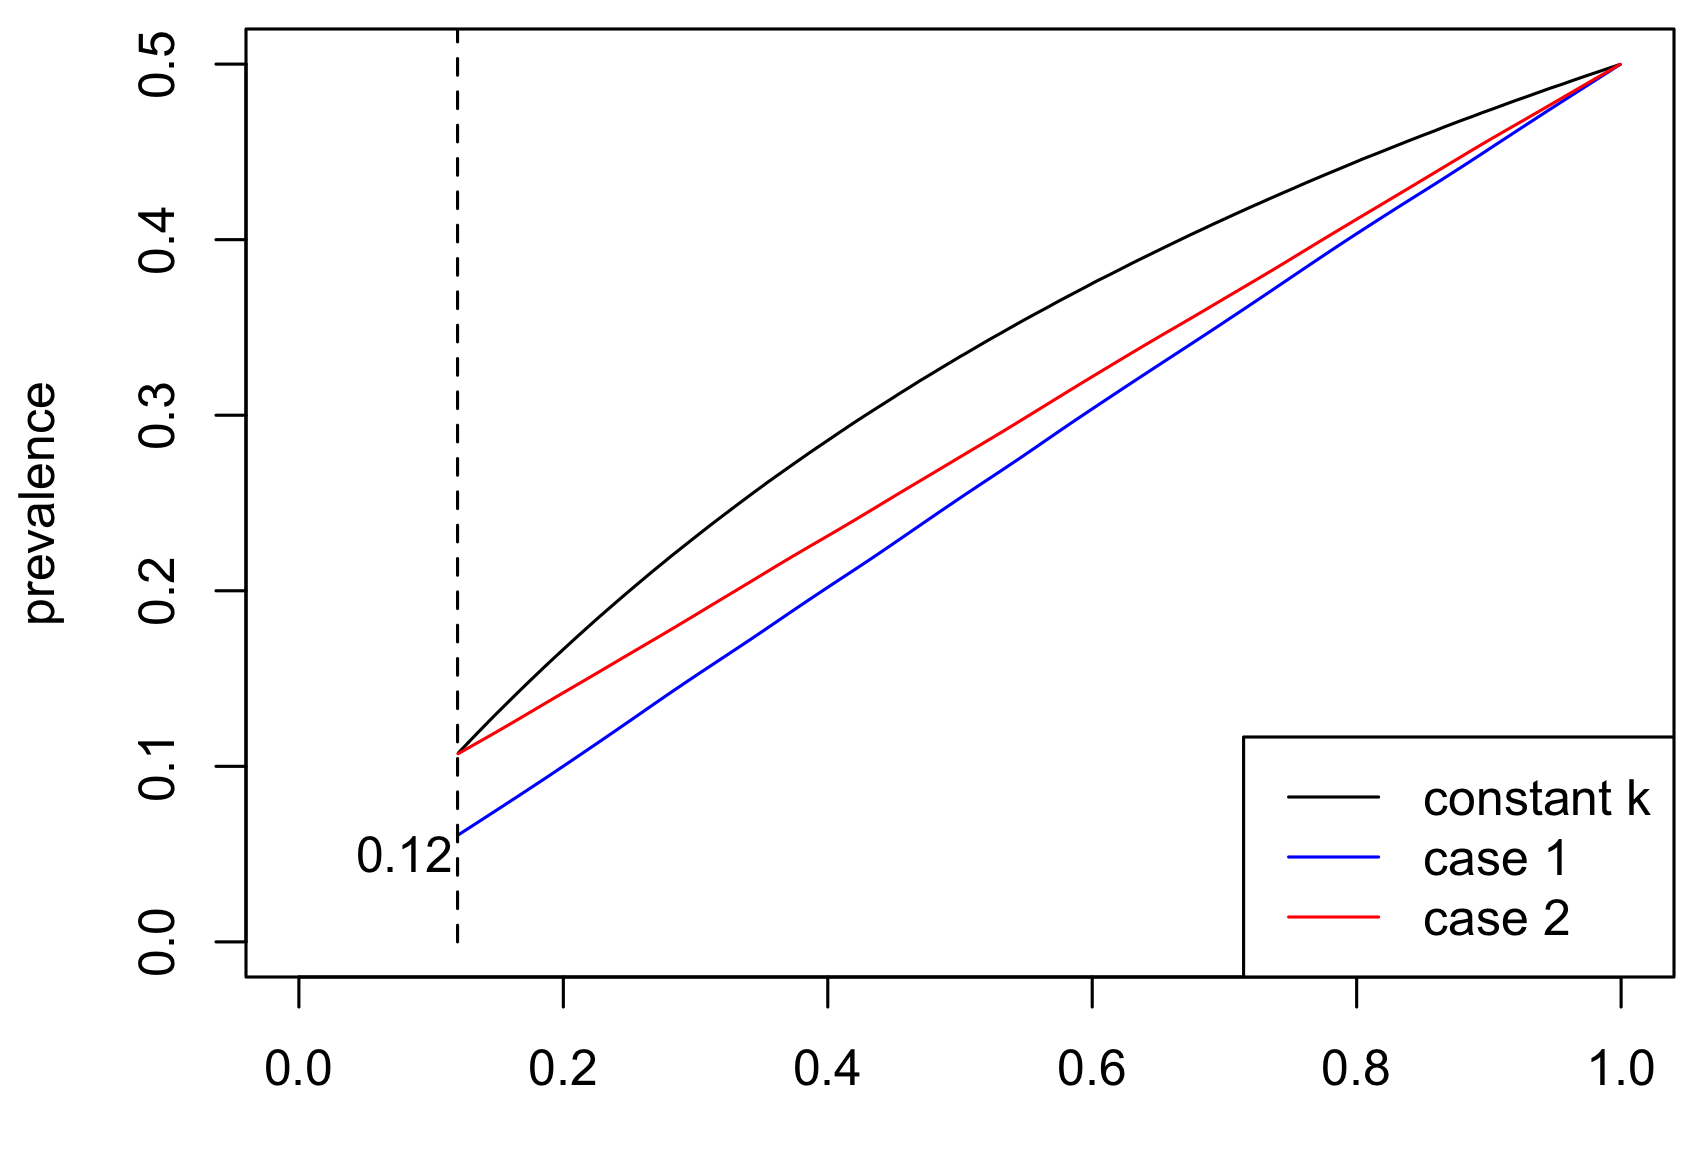
\includegraphics[width=7.45cm]{Figures/Aggregation/prevVmwb.png}
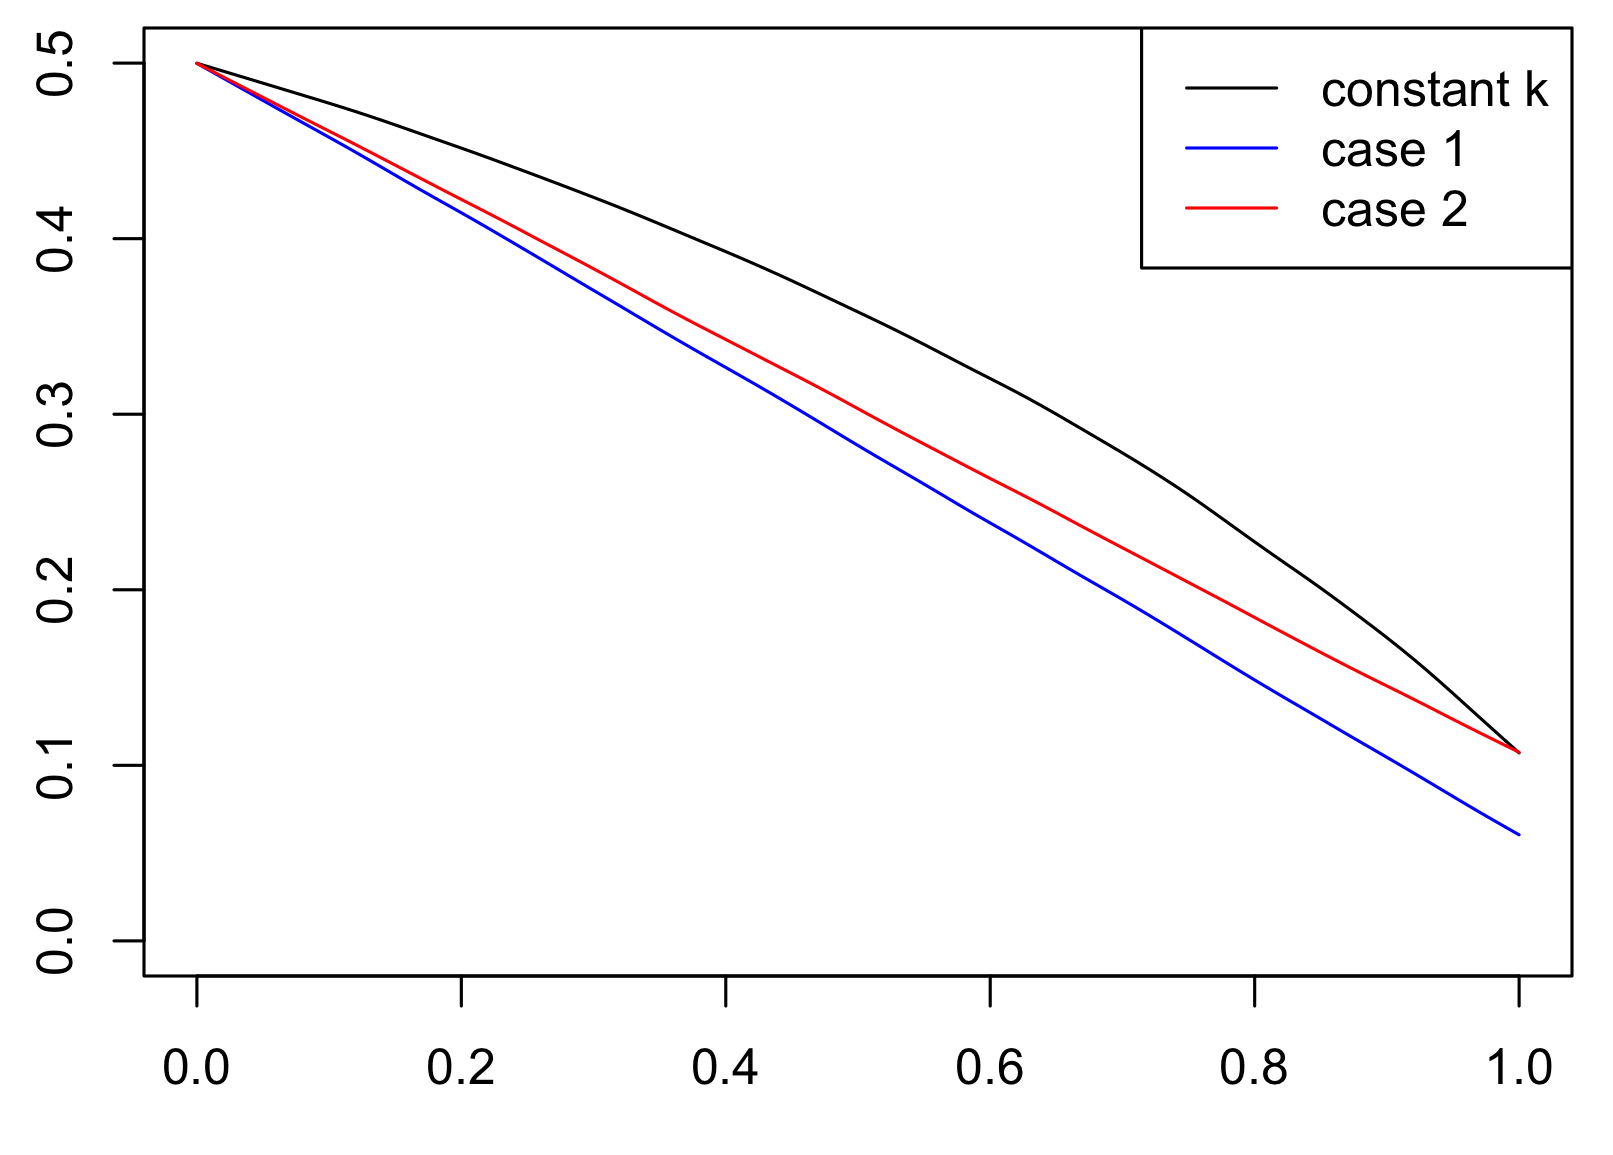
\includegraphics[width=7.1cm]{Figures/Aggregation/prevVmda.png}\\
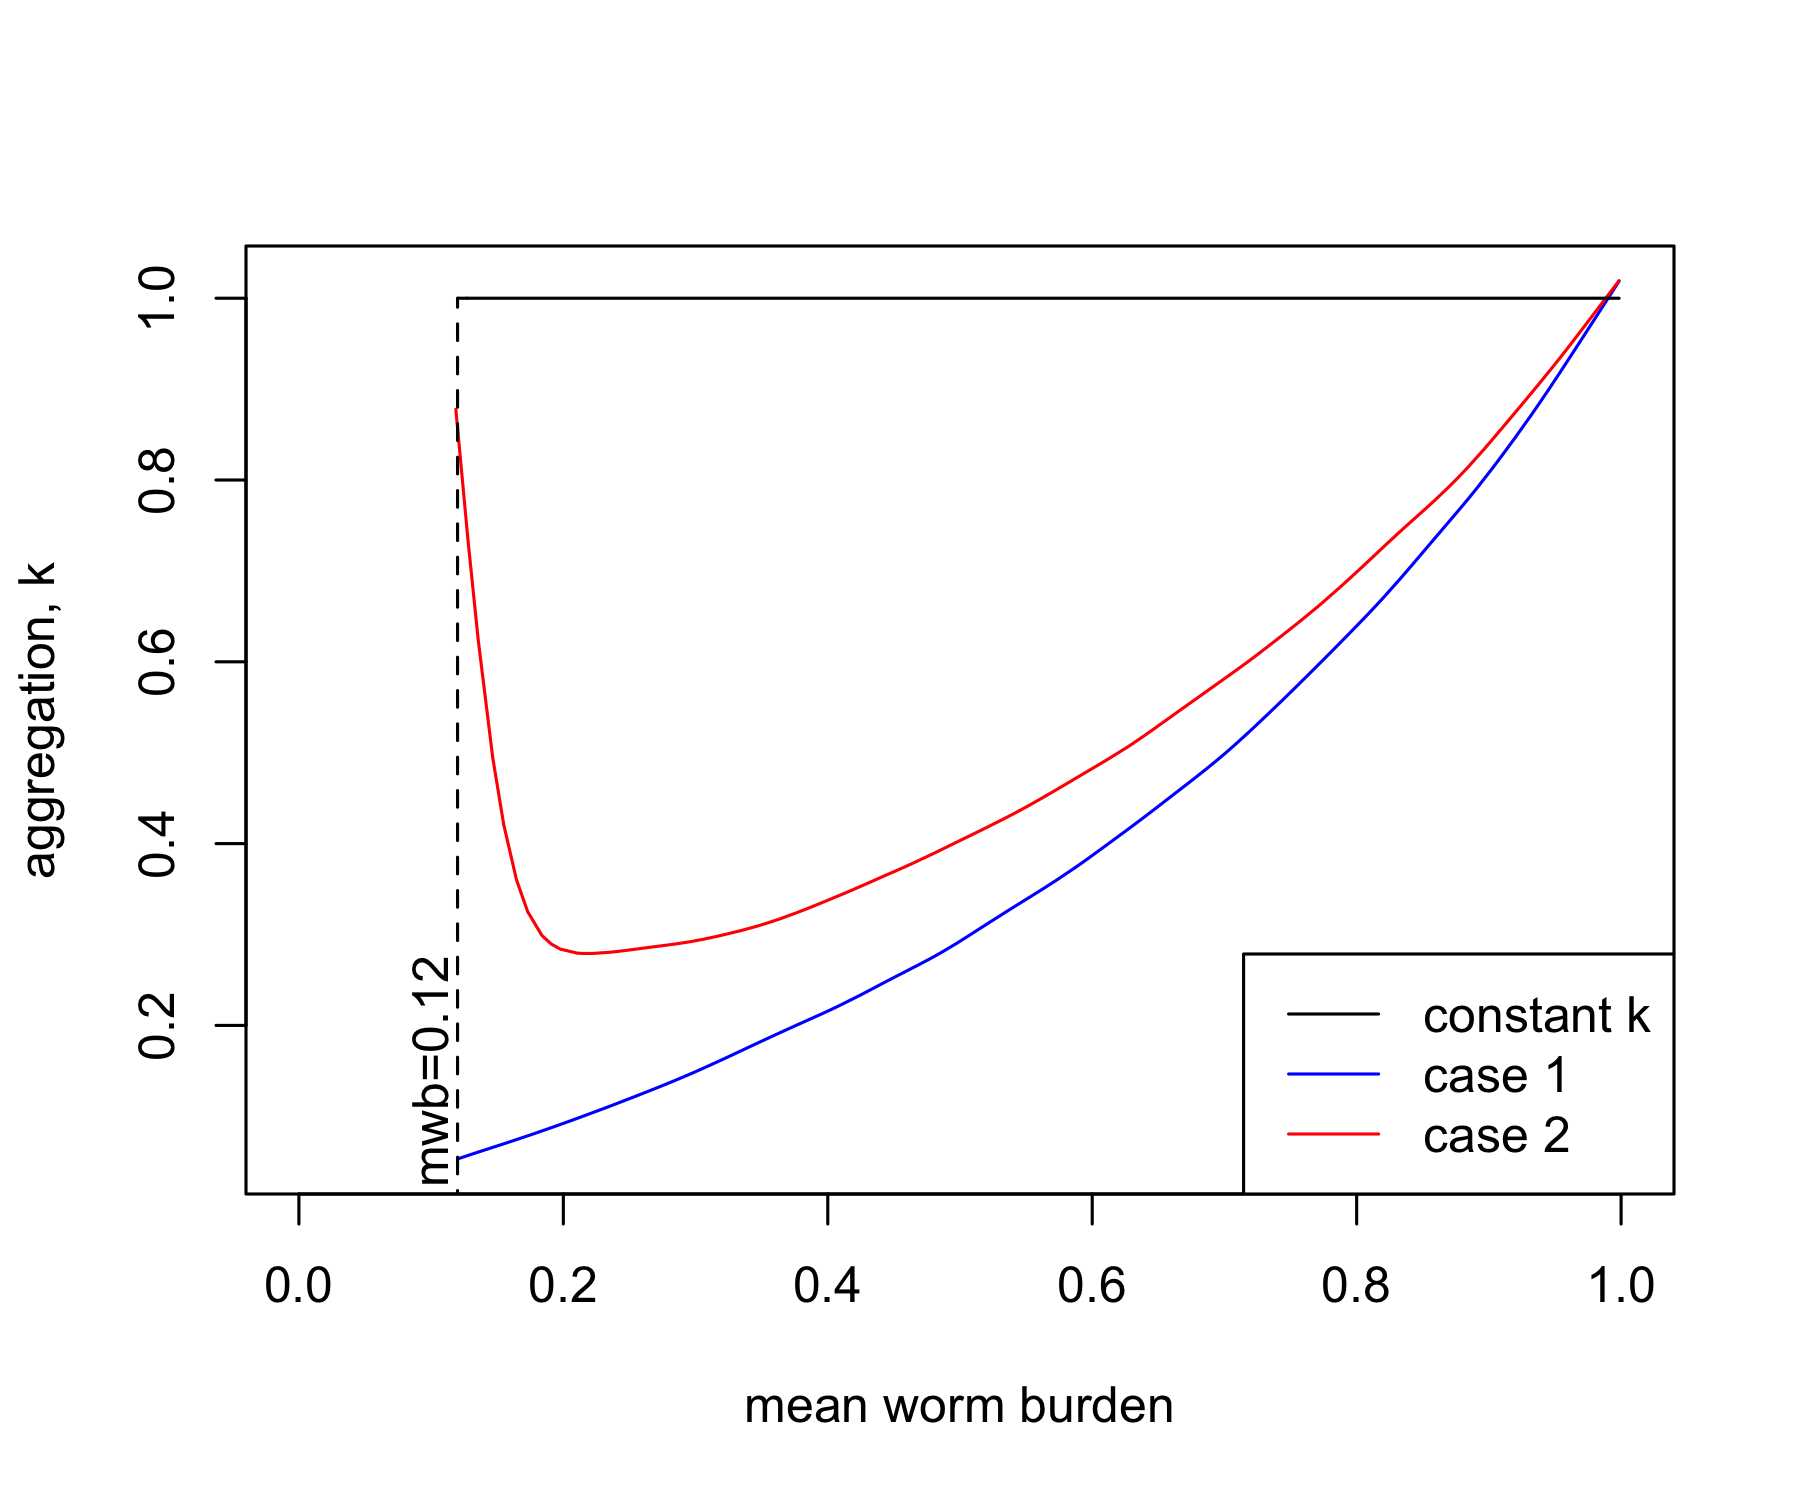
\includegraphics[width=7.45cm]{Figures/Aggregation/aggVmwb.png}
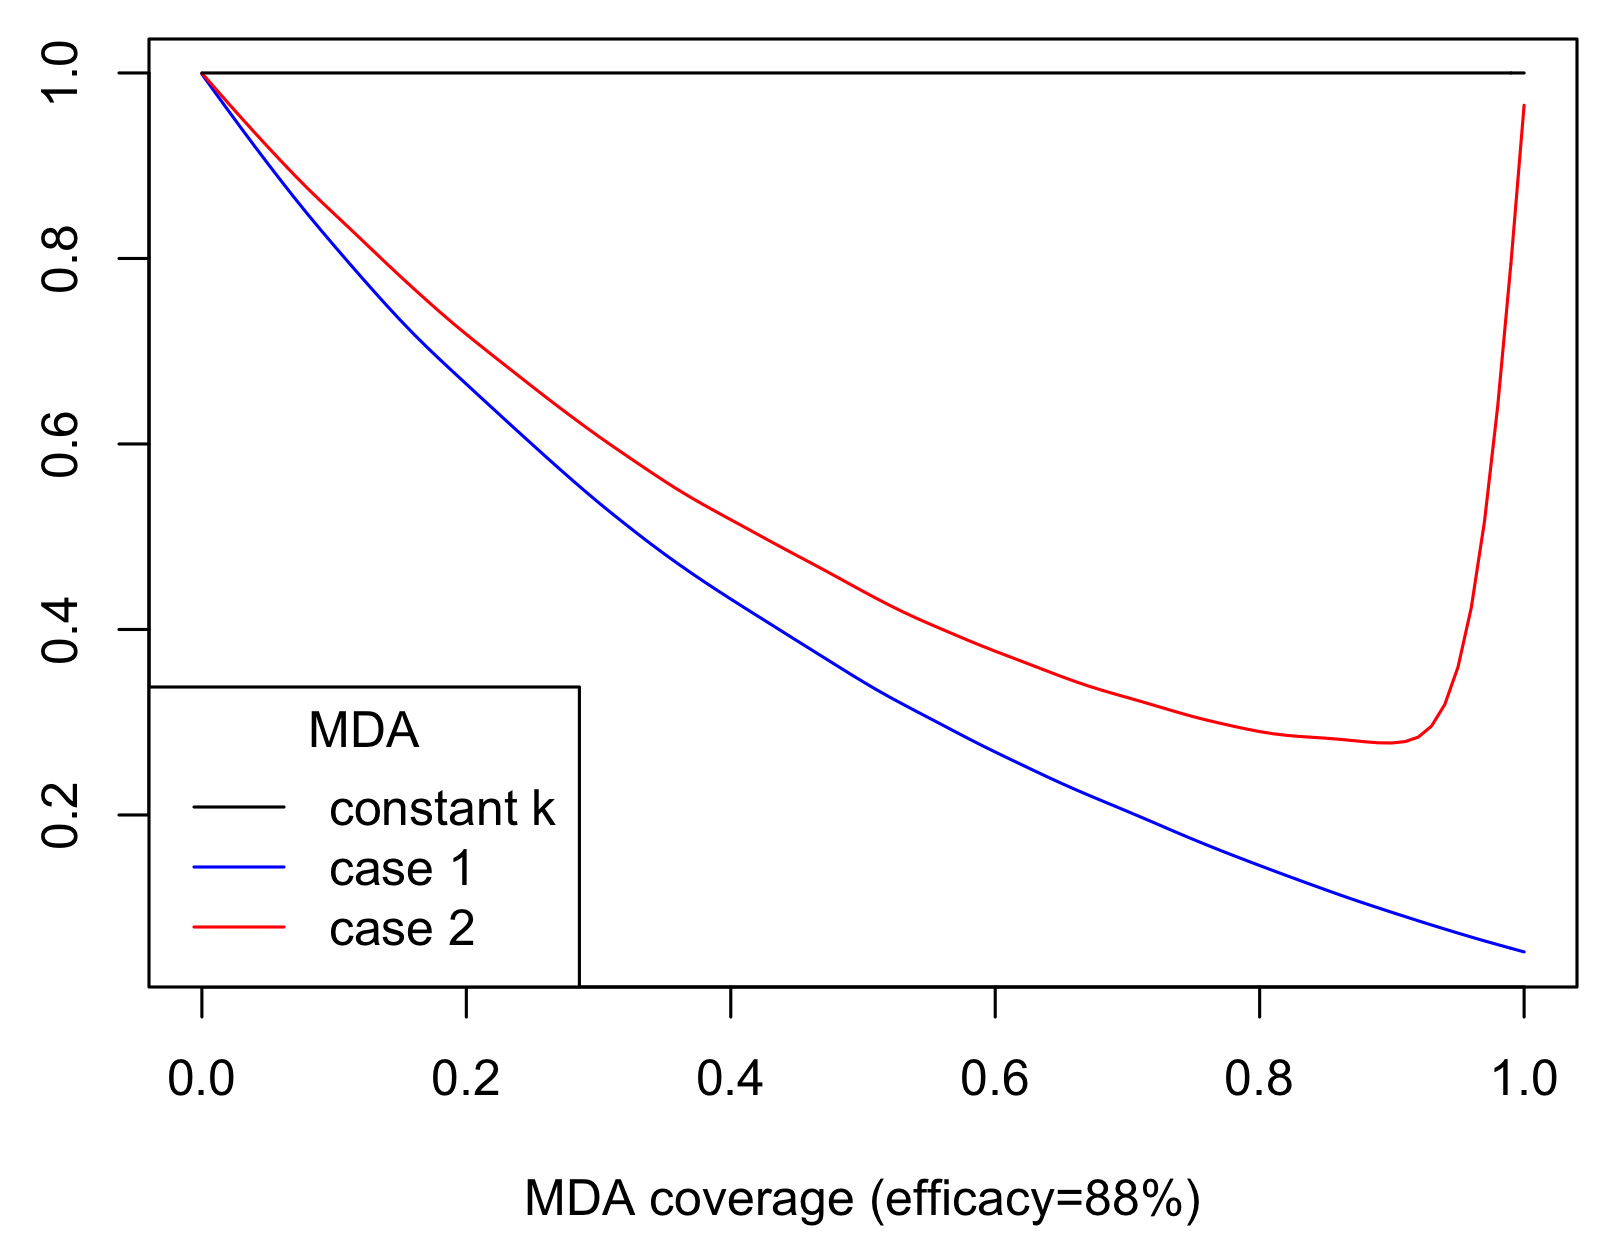
\includegraphics[width=7.1cm]{Figures/Aggregation/aggVmda.png}
\end{array}$
\caption[Aggregation and prevalence for different MDA assumptions.]{Relationships between mean worm burden, prevalence, parasite aggregation and MDA coverage for three cases: assuming MDA leads to proportional reduction of the mean with a constant aggregation parameter $k=1$ (black) and two cases of modelling one round of MDA coverage, with $k$ varied according to best fit negative binomial distribution. Case 1 (blue): MDA efficacy acts per person (either 0\% or 100\% of worms are cleared in each individual treated, with probability 0.88). Case 2 (red): MDA efficacy acts per worm (each worm in a treated human is cleared with probability 0.88). Host prevalence (top row) and parasite aggregation (bottom row) are given as functions of mean worm burden (left column) and MDA coverage (right column, efficacy $=88$\%).}
\label{fig:k}
\end{center}
\end{figure}

A negative binomial distribution is then fitted to the treated population and the new estimated value of the aggregation parameter, $k$, is recorded. Using this method we can numerically estimate $k$ for a range of mean worm burdens for both MDA assumption cases and then compare prevalence, using Equation \ref{eqn:negbin1}, to the population-level model using the constant value of $k$ (see Figure \ref{fig:k}). As the intervention modelled is one application of 88\% efficacy medication with a range of coverage between 0 and 100\%, the minimum possible resulting mean worm burden is 88\% less than baseline, which translates to a mean worm burden of 0.12.  

Our results show that assuming a constant $k$, and not re-fitting the negative binomial after applying an external force to the system, results in systematic over-estimation of prevalence compared to the individual-based model. Case 2 of modelling MDA (treatment efficacy per worm in each person treated) also results in a higher estimate of prevalence than Case 1 (treatment efficacy per person). This follows logically from the methods used, as assuming 100\% clearance in 88\% of cases treated will increase heterogeneity in worm burden and reduce prevalence.

We also see that the fitted aggregation parameter, $k$, varies dramatically with MDA coverage (and associated resulting mean worm burden). For Case 1 $k$ decreases with increasing MDA coverage and decreasing mean worm burden, and is close to zero at maximum coverage. This represents increasing heterogeneity as disease levels decline. Case 2 behaves similarly, albeit with a shallower gradient, until an MDA coverage of around 90\% (or a mean worm burden of around 0.2). At these high levels of coverage $k$ begins to increase again, representing reducing heterogeneity. As an effective coverage of higher than 90\% is infeasible in most settings \cite{Hussain2014,Babu2004}, with WHO recommended coverage of 65-80\% dependent on setting, this effect is interesting but has limited public health relevance.

\FloatBarrier

\subsection{Systematic non-adherence}

To consider the impact of extended MDA usage on aggregation we consider a sequence of four treatment rounds at a range of coverages (0-100\%), with the same initial conditions as before ($M=k=1$). Using Case 1 or Case 2 to model the MDA application, we can also consider the role of systematic non-adherence. We consider the two extreme cases: adherence is completely random, and adherence is completely systematic, i.e. the same individuals are treated in every round. 

\begin{figure}[h]
\begin{center}$
\begin{array}{cc}
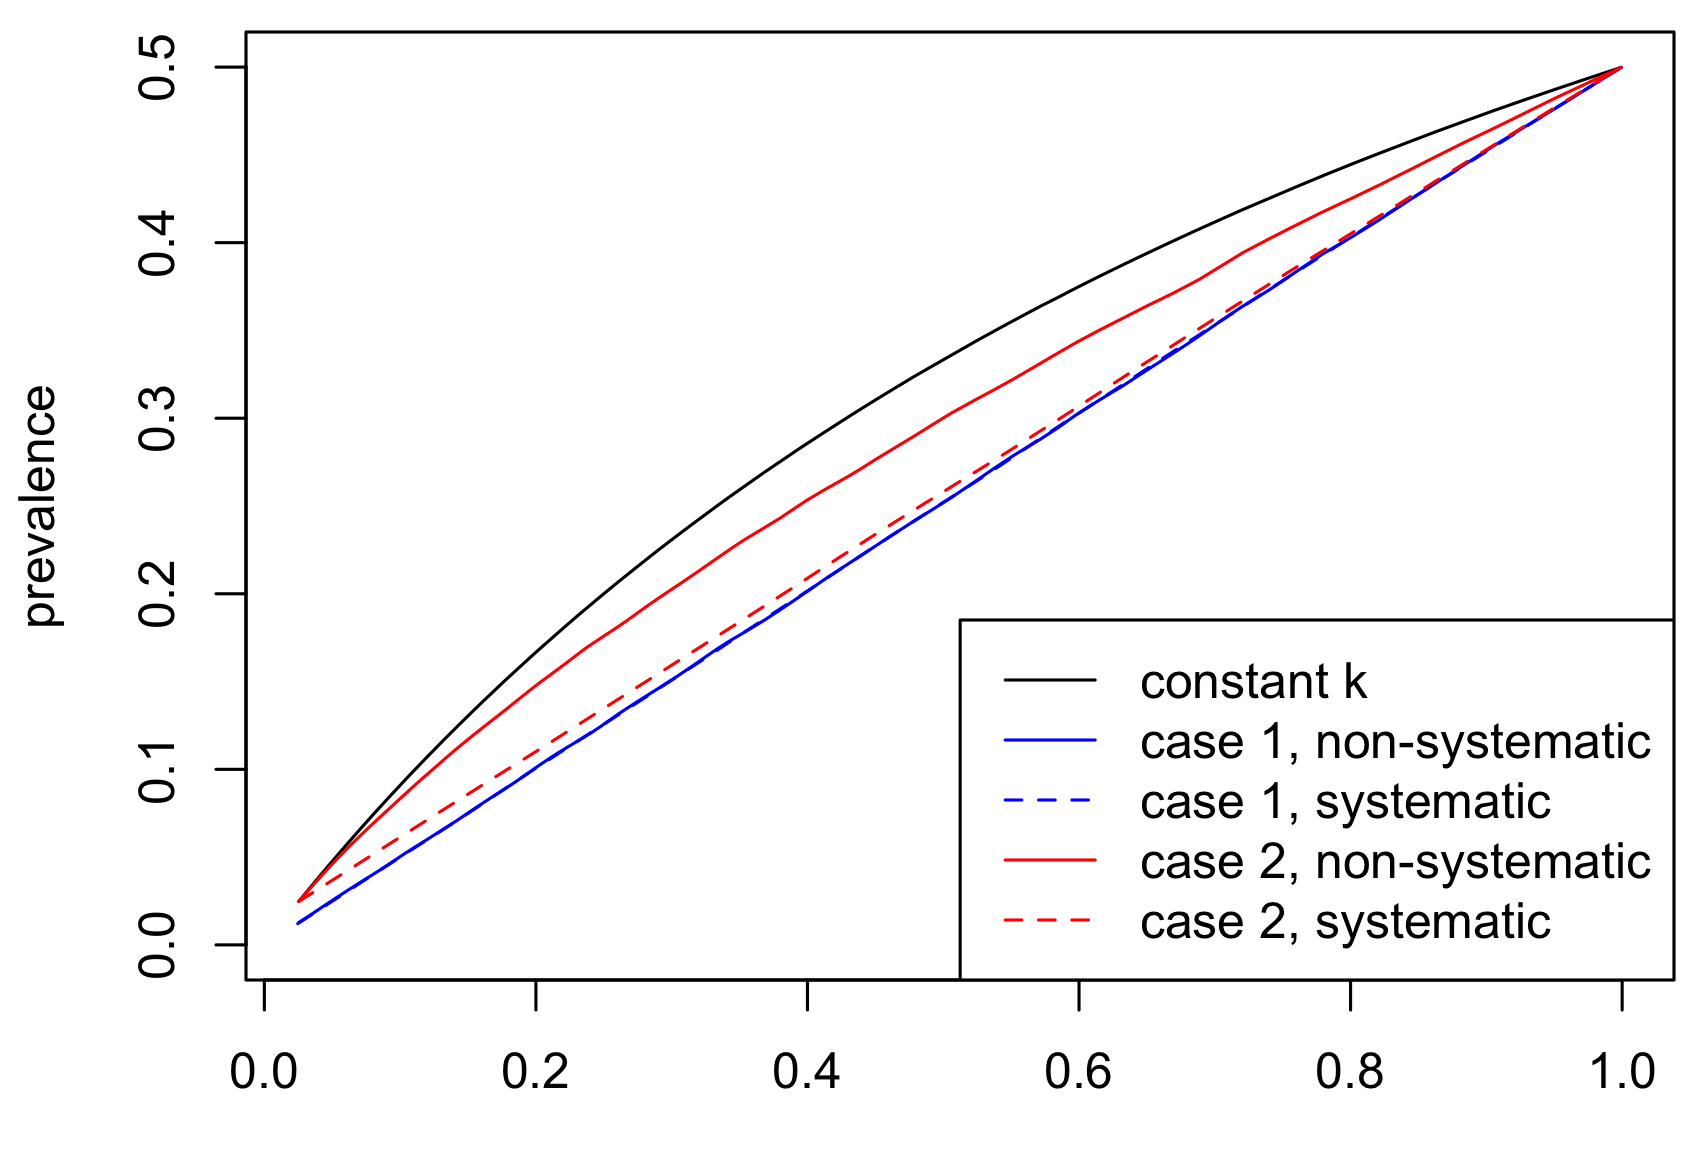
\includegraphics[width=7.45cm]{Figures/Aggregation/prevVmwb_Sys.png}
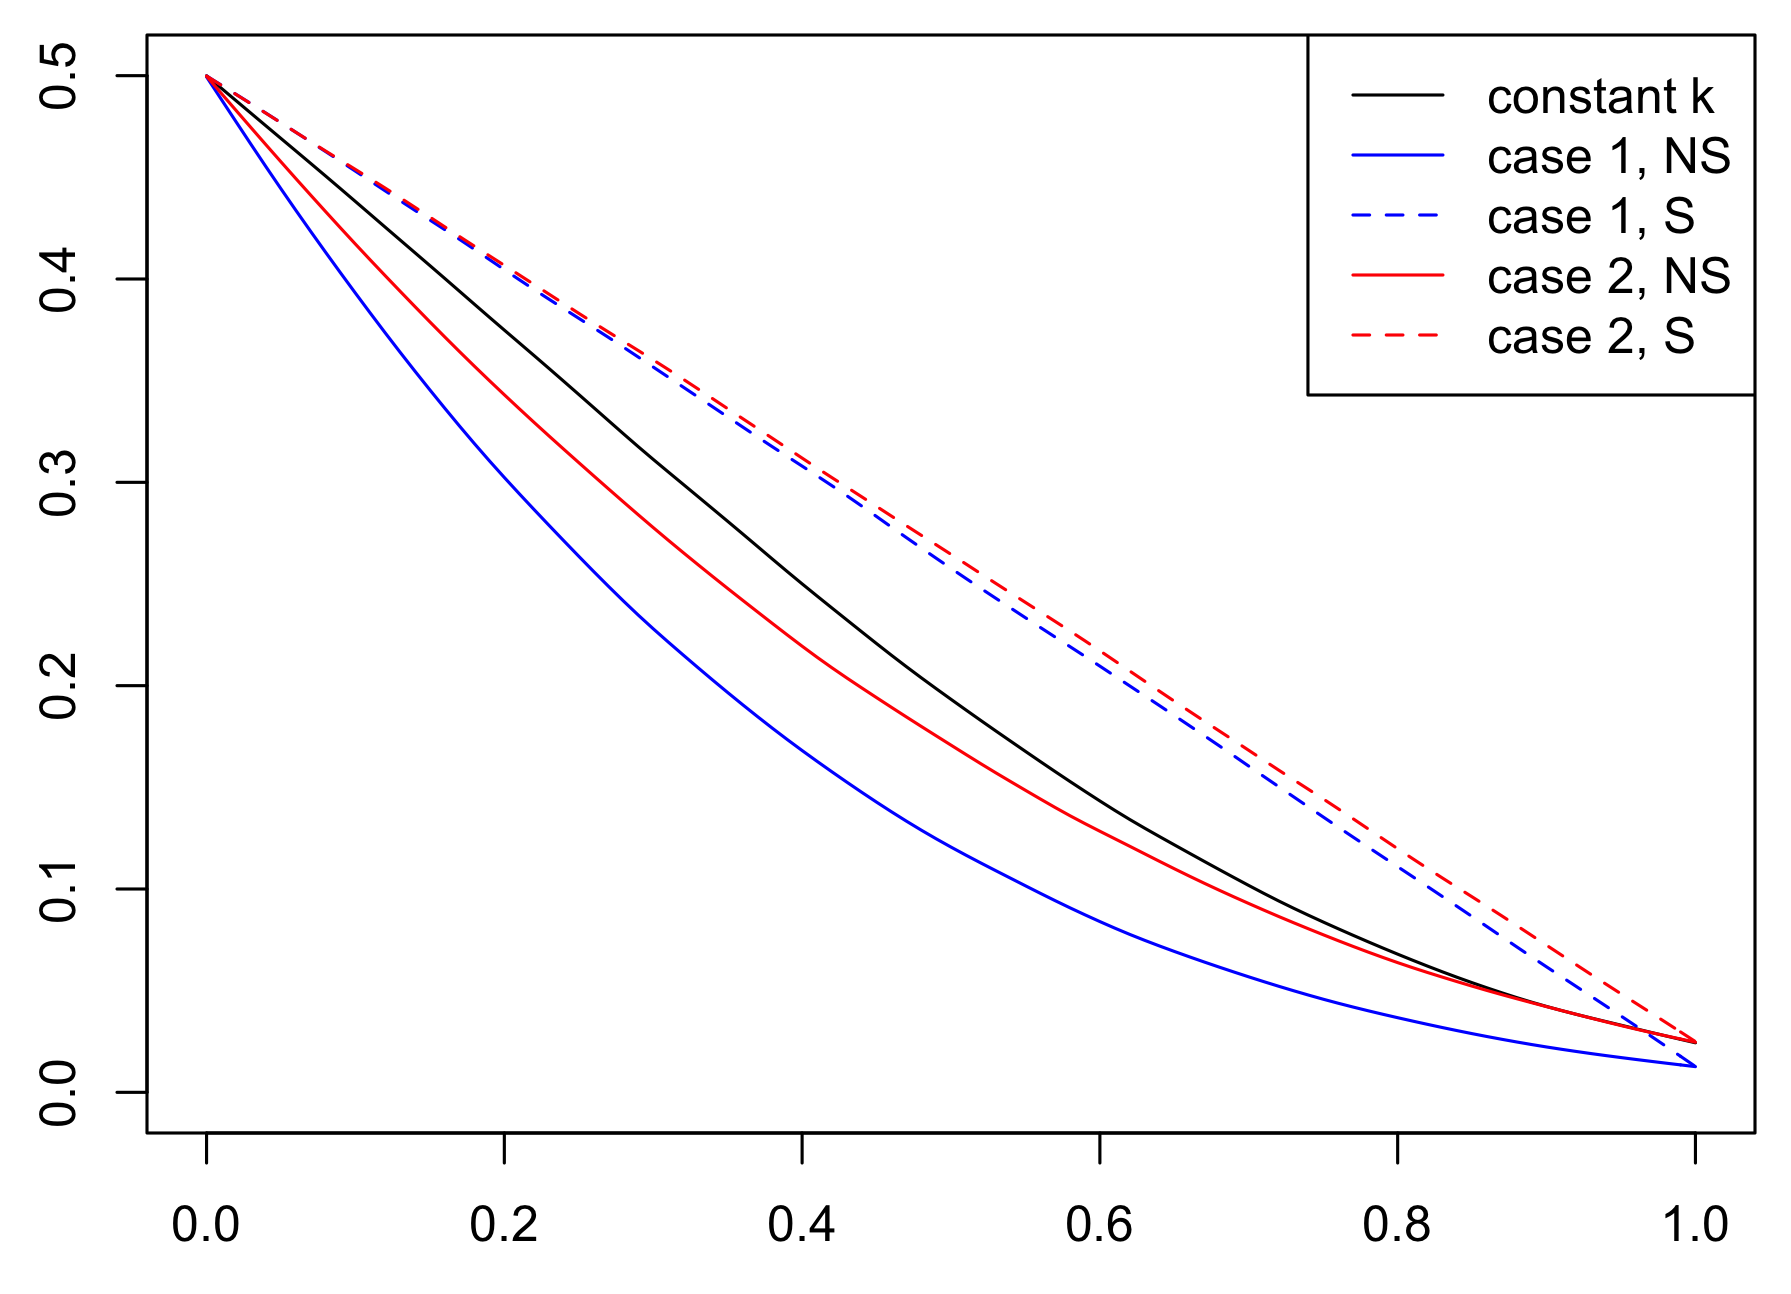
\includegraphics[width=7.1cm]{Figures/Aggregation/prevVmda_Sys.png}\\
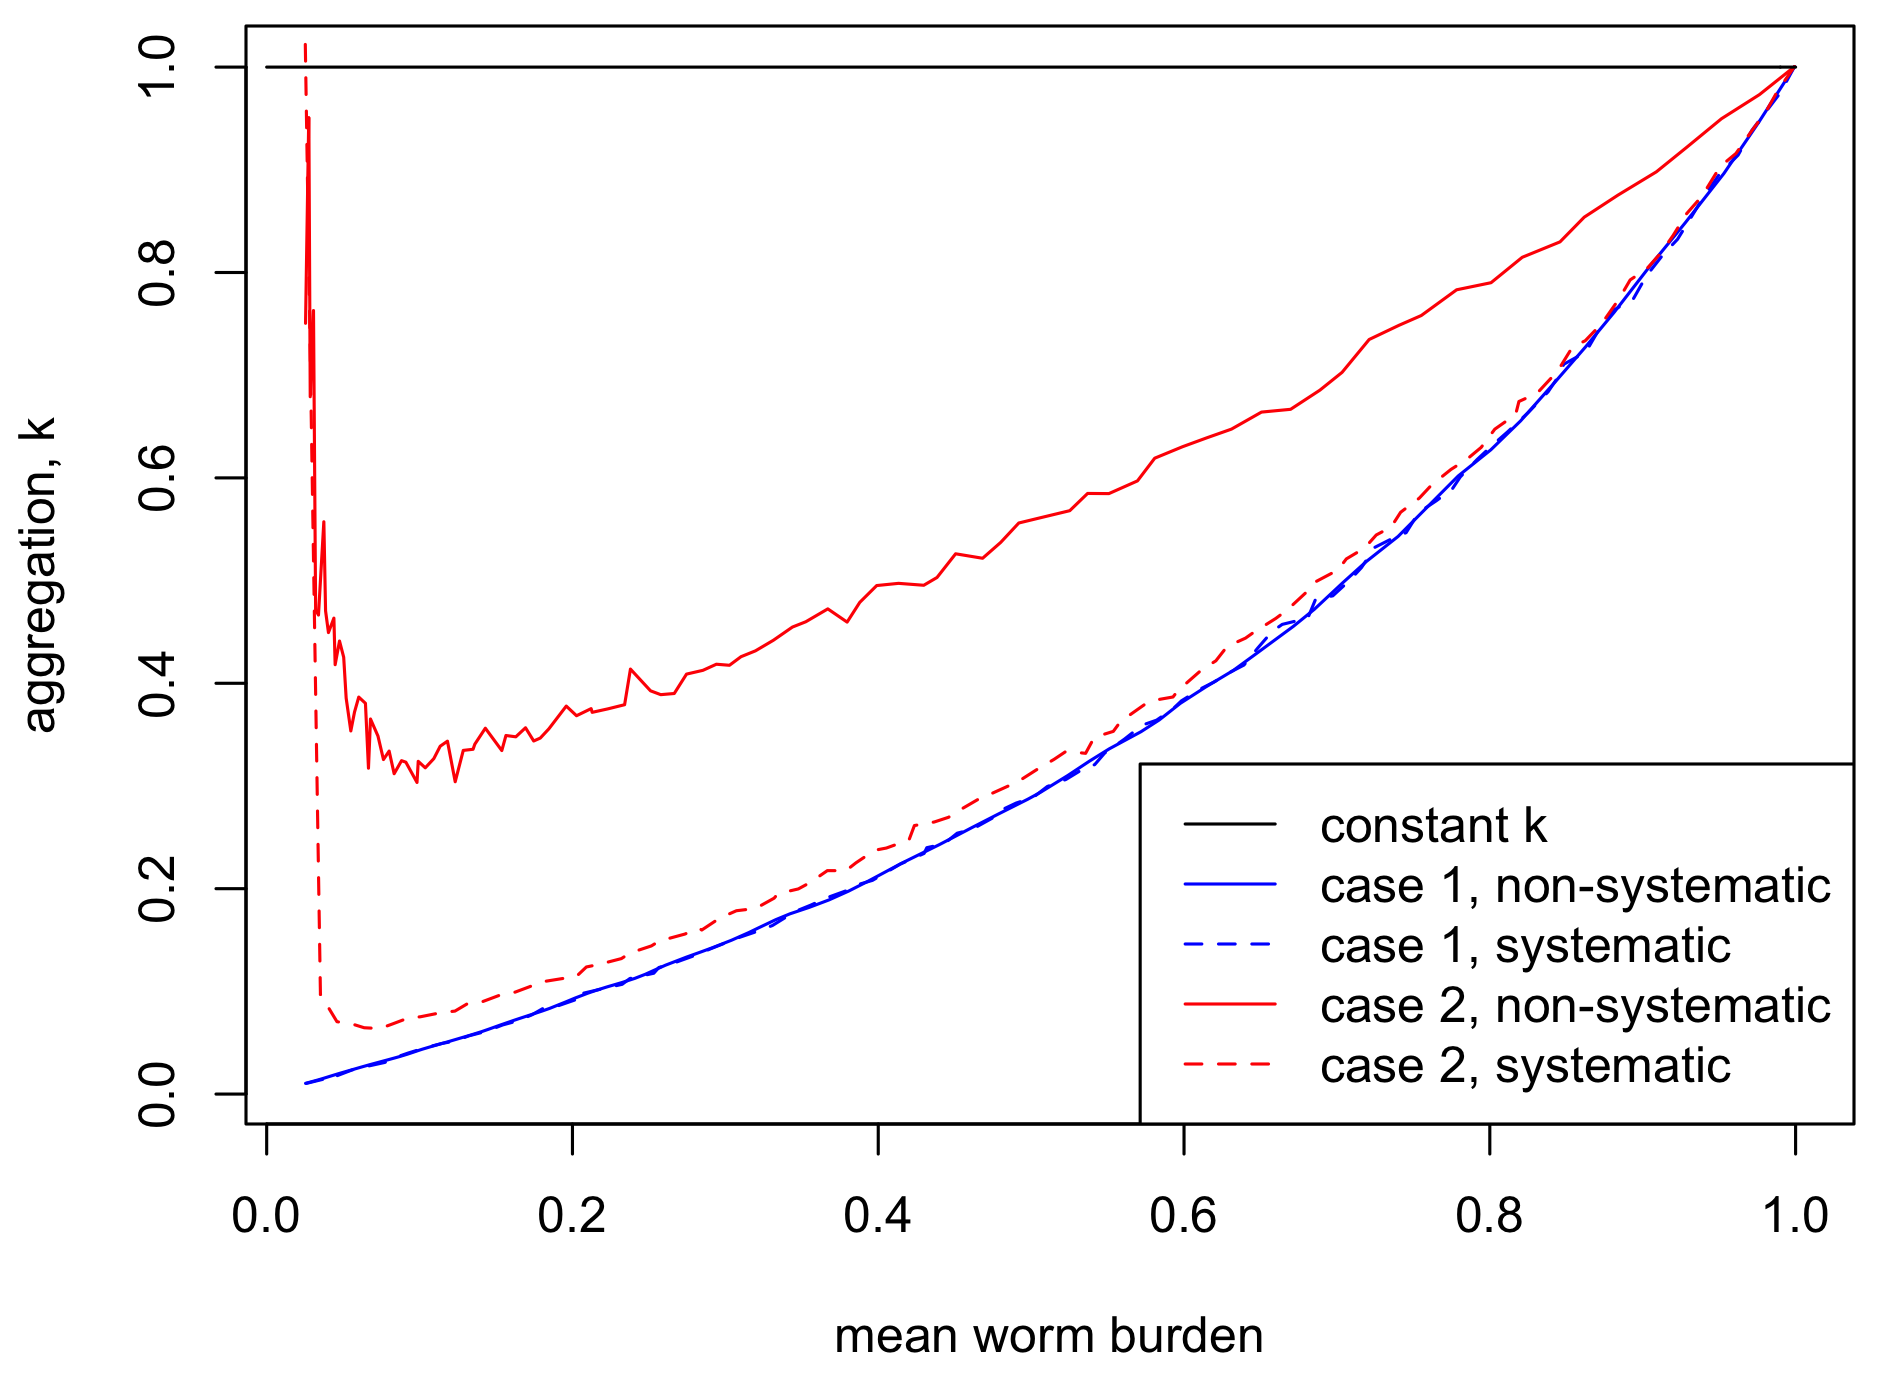
\includegraphics[width=7.45cm]{Figures/Aggregation/aggVmwb_Sys.png}
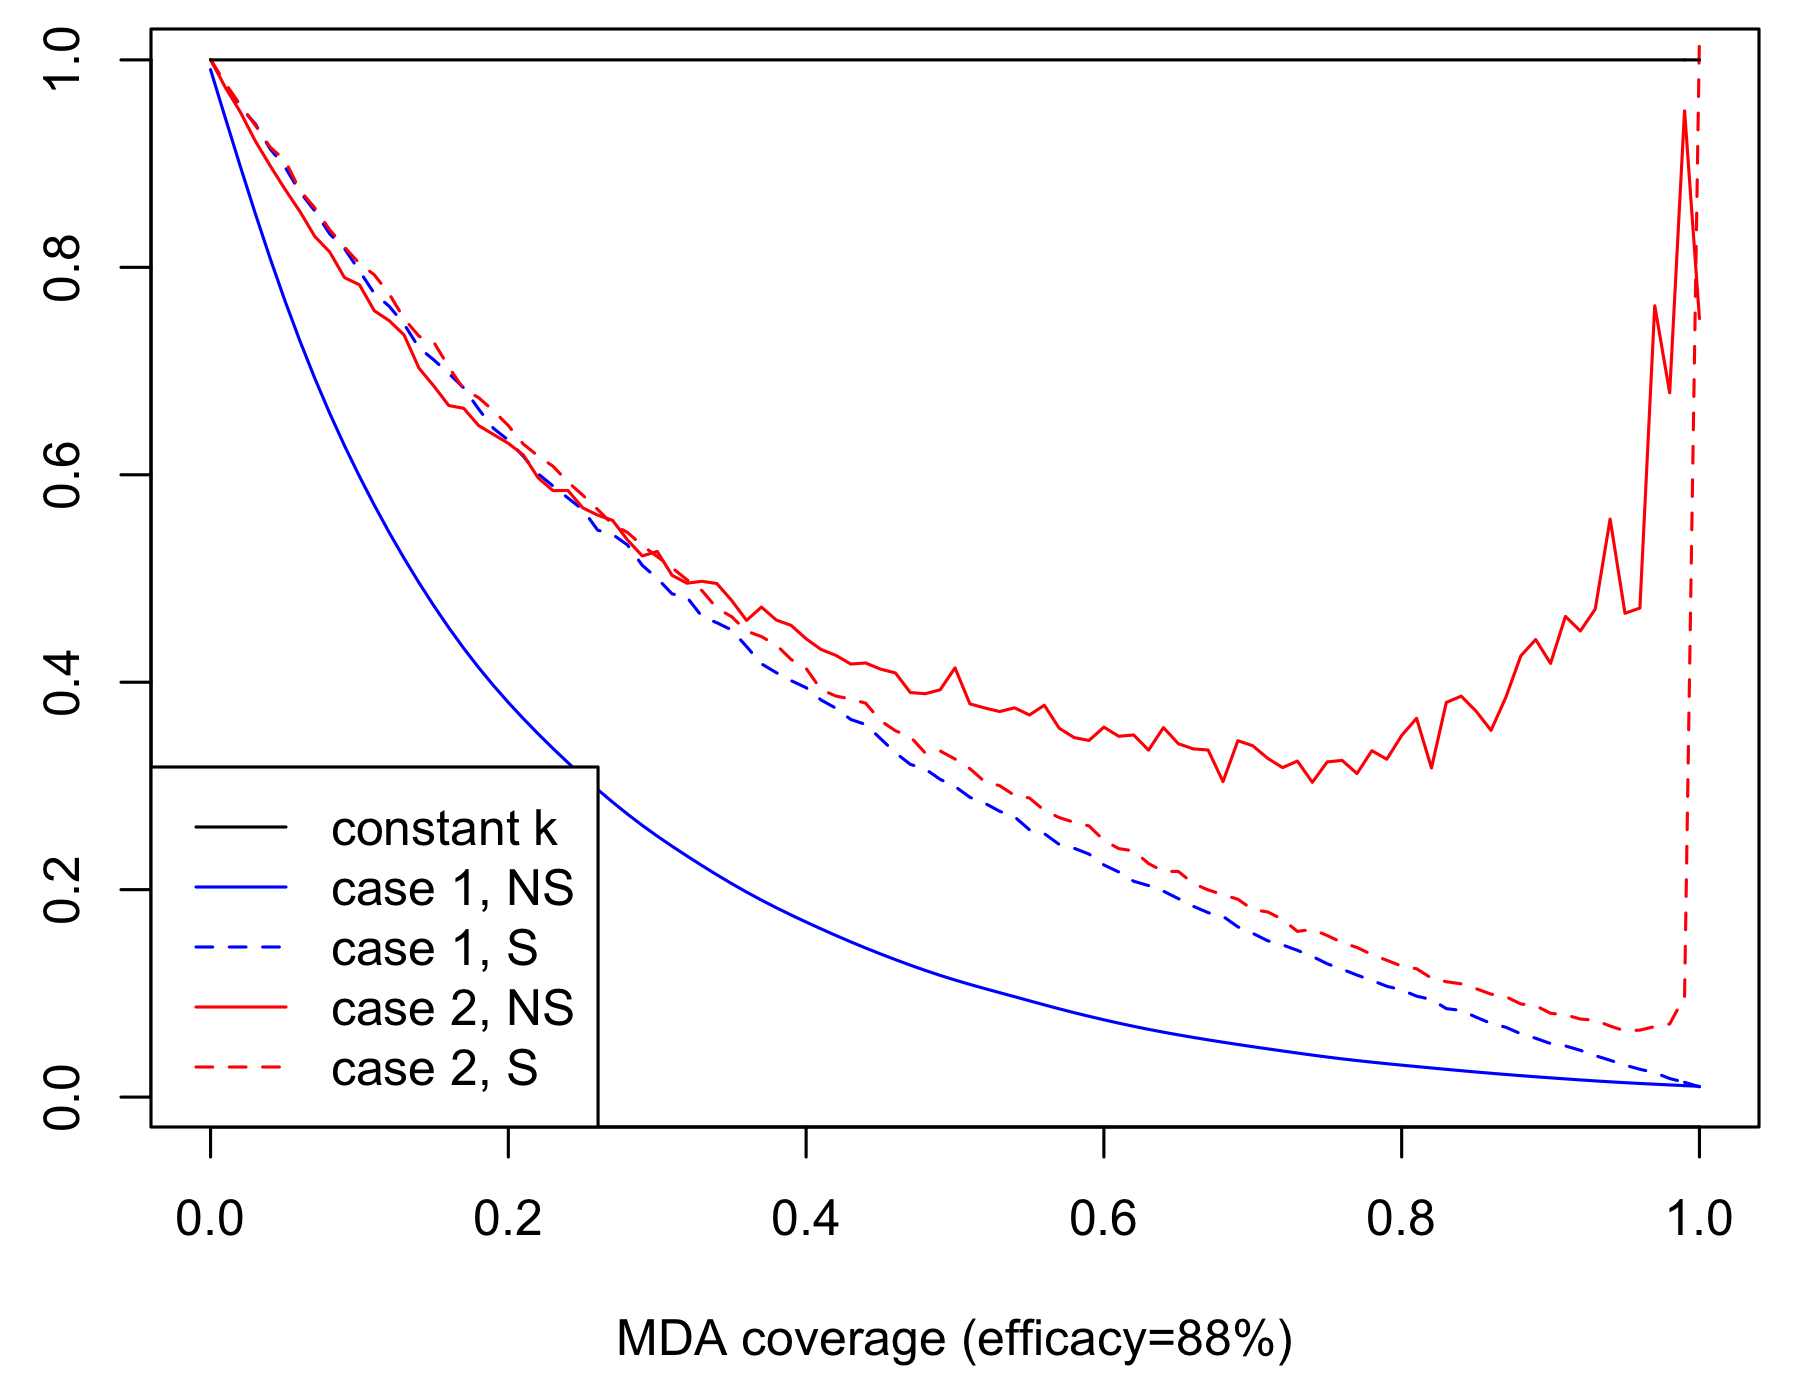
\includegraphics[width=7.1cm]{Figures/Aggregation/aggVmda_Sys.png}
\end{array}$
\caption[Aggregation and prevalence for systematic non-compliance.]{Relationships between mean worm burden, prevalence, parasite aggregation and MDA coverage for three cases: constant aggregation parameter $k=1$ (black), case 1 (blue) and case 2 (red) -- as described in Figure \ref{fig:k} --  after 4 rounds of MDA. Cases 1 and 2 are presented with random sampling (solid) and systematic non-compliance (dashed). Systematic non-compliance is taken to be maximal, with the same individuals missing treatment in each round. Host prevalence (top row) and parasite aggregation (bottom row) are given as functions of mean worm burden (left column) and MDA coverage (right column, efficacy $=88$\%).}
\label{fig:k_sys}
\end{center}
\end{figure}

Figure \ref{fig:k_sys} shows prevalence and $k$ for a range of MDA coverage and resulting mean worm burden. As expected, our results show that MDA programs with random adherence perform better than those with systematic adherence, due to a larger number of unique individuals treated. However, it's interesting to see that assuming random MDA coverage with treatment efficacy per worm leads to a substantially higher estimate of prevalence for the same mean worm burden than all other methods. The similarities between Case 1 and Case 2 in the case of complete systematic adherence implies that the reduction in aggregation caused by worm-based rather than human-based efficacy is overwhelmed by the increased aggregation caused by treating the same individuals each round. In all cases there are large discrepancies between the fitted estimates of prevalence and those calculated using a constant $k$. There is more noise in the non-systematic scenario of Case 2 than in other realisations because of the combined stochastic effects of randomly selecting both individual humans to treat and individual worms to clear in the presence of MDA, meaning a higher number of simulations would be required to achieve a comparably smooth curve.

\begin{figure}[h]
\begin{center}
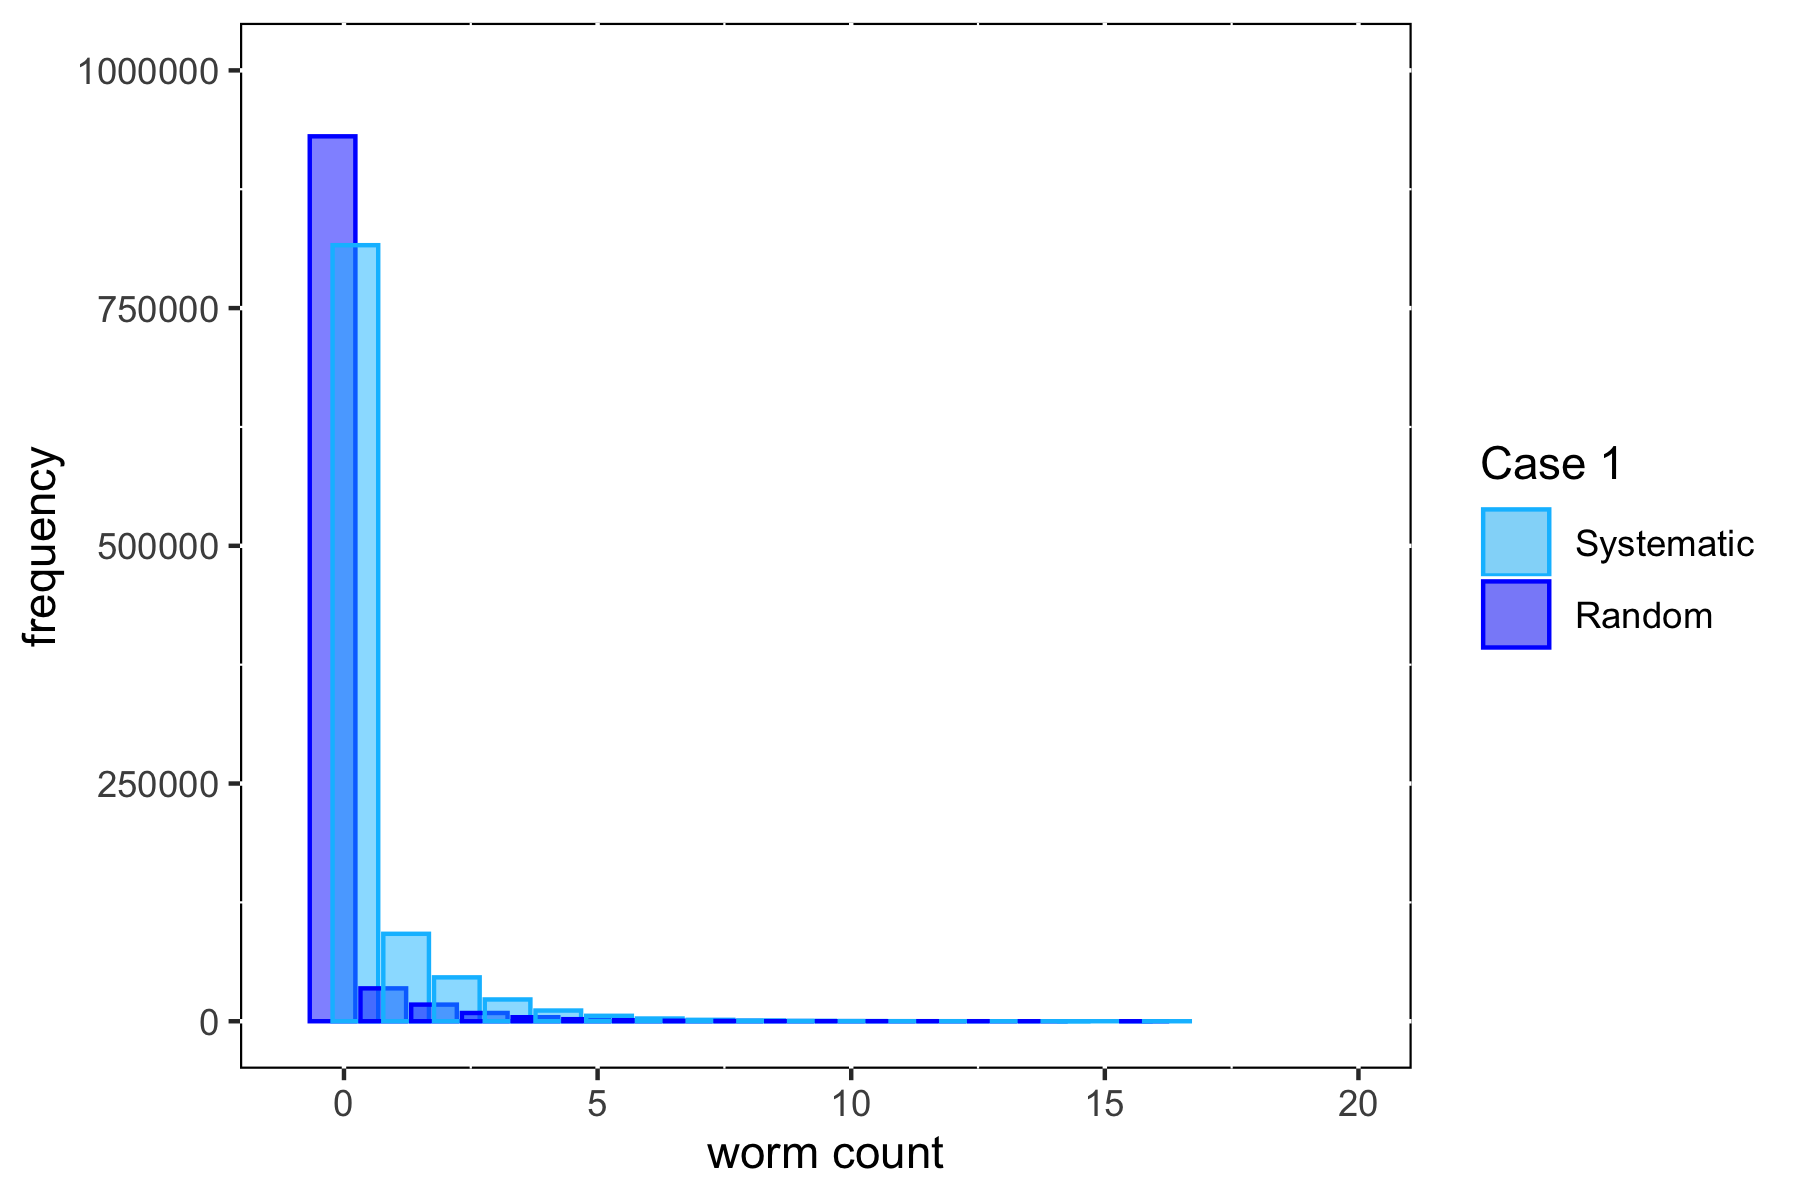
\includegraphics[width=12.5cm]{Project/Figures/Aggregation/Case1Hist.png}\\
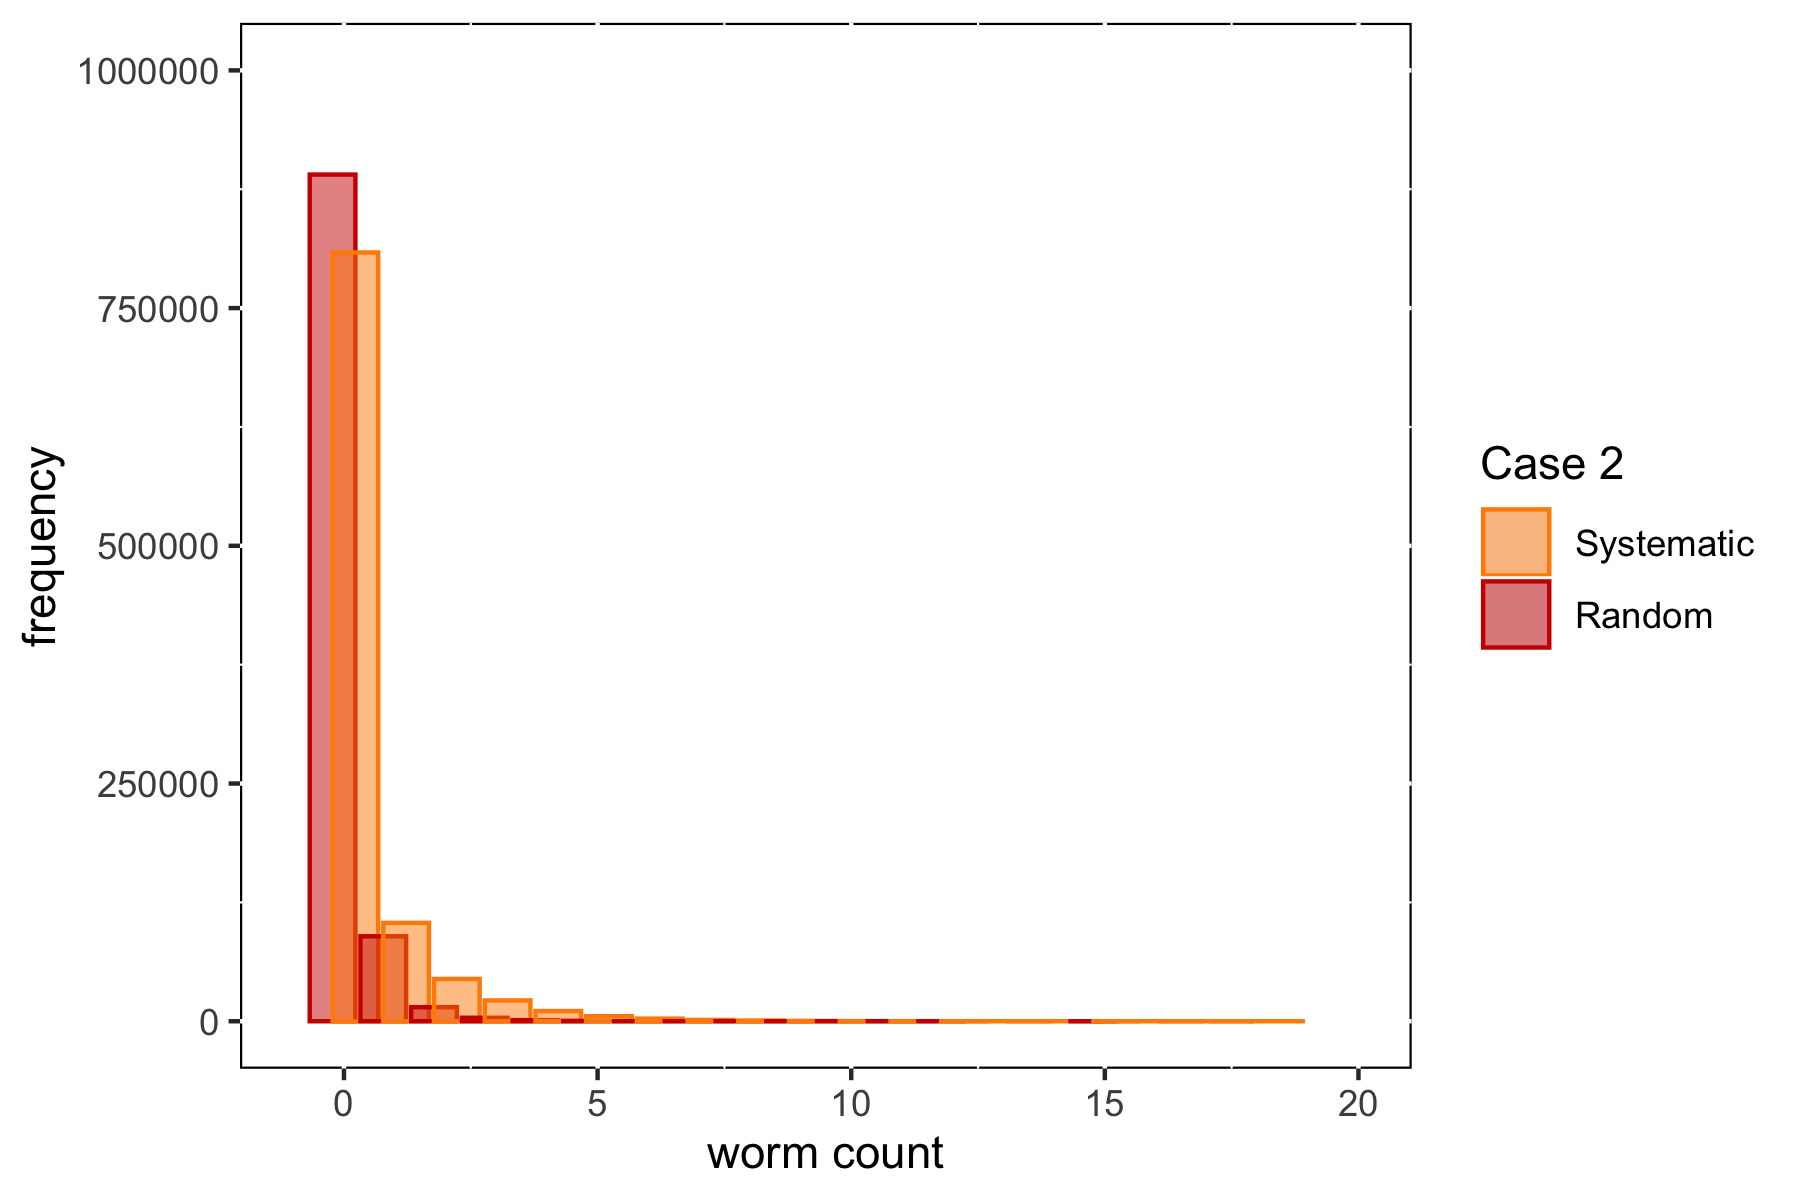
\includegraphics[width=12.5cm]{Project/Figures/Aggregation/Case2Hist.png}
\caption[Worm count frequency distributions.]{Example worm count frequency plots comparing systematic and random compliance for MDA cases 1 (Top, blue, drug efficacy per host) and 2 (Bottom, red, drug efficacy per worm). Worm counts are taken after 4 rounds of MDA at 65\% coverage in each case. MDA efficacy $=$ 88\%.}
\label{fig:kHist}
\end{center}
\end{figure}

Figure \ref{fig:kHist} depicts example worm count frequencies comparing systematic and random adherence across the two MDA modelling methods, assuming a coverage of 65\%. In both cases we see a decrease in the number of zeros and an overall increase in heterogeneity when we assume systematic adherence. Looking back at Figure \ref{fig:k_sys} we see that at 65\% MDA coverage there is a similar distance between systematic and random aggregation estimates for both cases, explaining the similarities between these two histograms.

\FloatBarrier

\section{Concluding remarks}

Using a simple individual-based formulation of parasite infection, I have shown that assuming a negative binomial relationship between mean worm burden and prevalence with constant aggregation, $k$, may not always be appropriate. In particular, MDA and the way it is modelled is likely to have effects on this relationship that cannot be characterised by a constant aggregation assumption. The relationships shown also demonstrate complex relationships between aggregation, MDA coverage, mean worm burden and prevalence. This implies that expressing $k$ as a linear function of mean worm burden may also be insufficient to capture changes in the underlying parasite distribution caused by external pressures.

We find that both systematic compliance and MDA assumptions have an impact on estimated distribution parameters and the associated aggregation, with systematic non-adherence resulting in potentially large changes in prevalence and aggregation estimates. These results highlight the importance of caution when translating between mean worm burden and prevalence across all helminth infections, as well as the need for further biological and modelling studies in the characterisation of these relationships.

\subsection{Chapter summary}

In this chapter I used an individual-based model to investigate the relationship between disease prevalence and infection intensity for helminth parasites, in particular focusing on analysis of the commonly-made negative binomial assumption. Considering a range of possible modelling assumptions, I demonstrated that assuming constant or linear values of the aggregation parameter, $k$, could potentially be inappropriate in a number of scenarios, resulting in an over-estimation of prevalence and an under-estimation of aggregation.